\documentclass[a4paper,12pt]{article}

 \addtolength{\oddsidemargin}{-.5in}
\addtolength{\evensidemargin}{-.5in}
\addtolength{\textwidth}{1.0in}
\addtolength{\topmargin}{-.5in}
\addtolength{\textheight}{1.0in}


\usepackage{graphicx}
\usepackage{amsmath}
\usepackage{amssymb}
\usepackage{amsthm}
\usepackage{xcolor}
\usepackage{color}
\usepackage{bbding}
\usepackage{algorithm}
\usepackage[noend]{algpseudocode}
\newtheorem{theorem}{Theorem}
\newtheorem{corollary}{Corollary}

\begin{document}

\title{Group 4: The Kaczmarz Algorithm}
\author{Wei Deng, Nicole Eikmeier, Nate Veldt, and Xiaokai Yuan}
\maketitle{}


\section{Introduction}
Project Objective:

Given a large sparse linear system $Ax = f$, of order $n = 10^6$ that can be effectively reduced to a banded matrix using the reordering scheme ``reverse Cuthill-McKee", use the method of Row Projection, accelerated via the Conjugate Algorithm to yield a parallel solver. Compare the robustness and parallel scalability/speed with preconditioned Krylov subspace methods preconditioned via approximate LU-factorization.

\vspace{.2in}

The Kaczmarz Algorithm is a row projection method which is equivalent to solving $AA^Ty = f$ using the Gauss-Siedel iteration, with $x = A^Ty$. In Kaczmarz we consider each equation as a hyperplane:
$$S_i=\{x:A_ix-b_i=0\}$$ for $i=1,2,...$, where $A_i$ and $b_i$ are $i$th row of matrix $A$ and vector $b$. So the problem is transformed into finding the coordinates of the point of intersection of these hyperplanes.  See figure \ref{fig:ClassKacz} for a visualization of the problem.

\begin{figure}[htbp]
\begin{centering}
%\begin{minipage}[b]{0.8\linewidth}
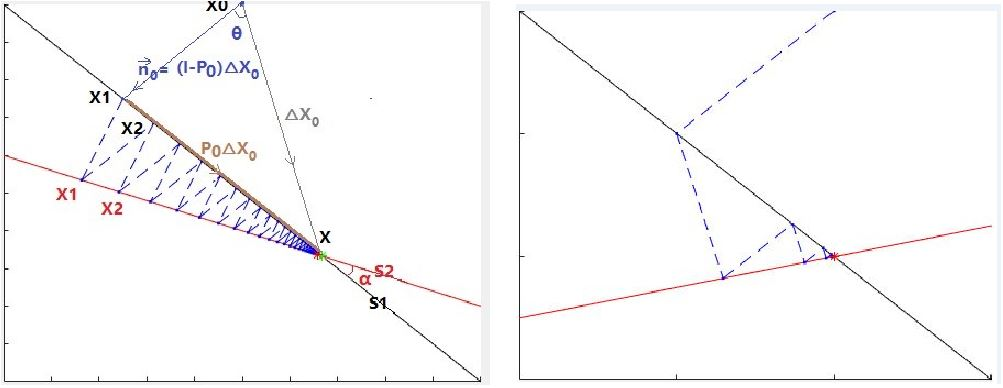
\includegraphics[width=5in]{Images/Classical_Kaczmarz}
\caption{2-Partition Case of the Kaczmarz Algorithm}
\label{fig:ClassKacz}
%\end{minipage}
\end{centering}
\end{figure}

From this basic idea we use symmetrization and acceleration via the CG method to improve the procedure. The details will be given carefully in the following sections.




\section{Implementation}


%------------------------------------------------
%------------------------------------------------
% REVERSE CUTHILL-MCKEE
%------------------------------------------------
%------------------------------------------------

\subsection{Reverse Cuthill-McKee and the Woodbury Formula}
The first step in our implementation is to transform the sparse matrix $A$ to a banded form using Reverse Cuthill-McKee. We can perform a symmetric permutation with matrix $P$ so that $P^TAP$ is banded. In figure \ref{fig:v3}, we see the result from Matlab of Reverse Cuthill Mckee on the stomach data set. The band size is nice and small.

%\begin{figure}[ht]
%\centering
%\begin{minipage}[b]{0.45\linewidth}
%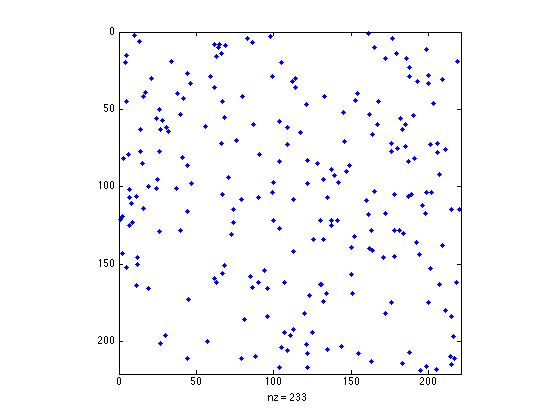
\includegraphics[width=2in]{Images/SparseA.jpg}
%\caption{$A$ sparse, non-symmetric}
%\end{minipage}
%\quad
%\begin{minipage}[b]{0.45\linewidth}
%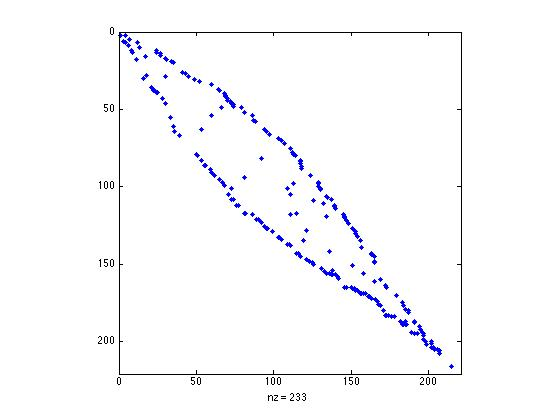
\includegraphics[width=2in]{Images/Arcm.jpg}
%\caption{$P^TAP$ (banded)}
%\label{fig:banded}
%\end{minipage}
%\end{figure}

\begin{figure}[ht]
\centering
\begin{minipage}[b]{0.45\linewidth}
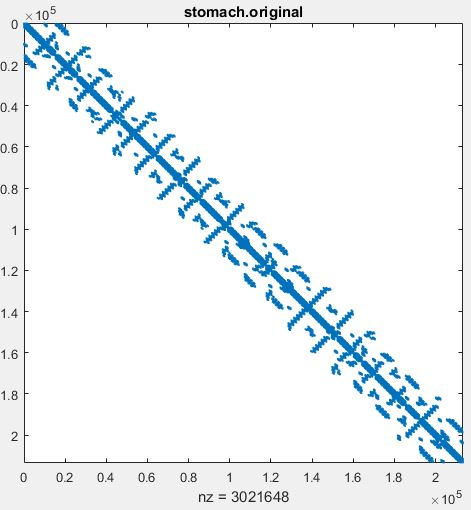
\includegraphics[width=2in]{Images/SparseA_v5.jpg}
\caption{$A$ sparse, non-symmetric}
\label{fig:v5}
\end{minipage}
\quad
\begin{minipage}[b]{0.45\linewidth}
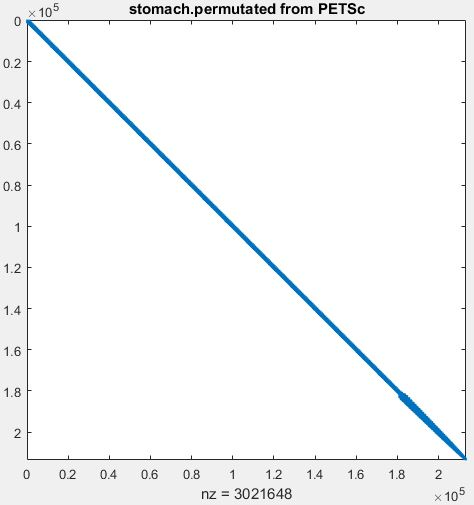
\includegraphics[width=2in]{Images/Arcm_v3.jpg}
\caption{$P^TAP$ (banded)}
\label{fig:v3}
\end{minipage}
\end{figure}

For some problems the bandwidth could be too large after using Reverse Cuthill Mckee. See for example figure \ref{fig:approxbanded}, where we see the result of RCM on the lns$\_$131 data set, again in Matlab.  If this is the case, instead we could choose $P$ so that $P^TAP$ is narrow banded plus a low rank matrix. See figure \ref{fig:woodbury}. 

\begin{figure}[ht]
\centering
\begin{minipage}[b]{0.45\linewidth}
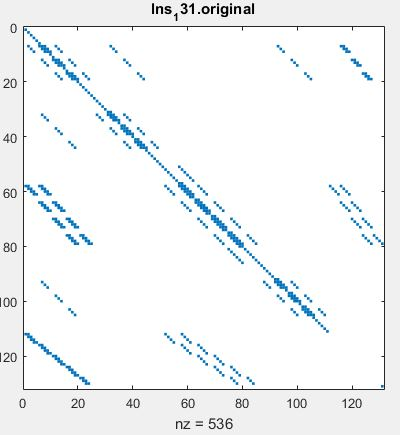
\includegraphics[width=2in]{Images/SparseA_v4.jpg}
\caption{$A$ is sparse and non-symmetric}
\label{sparseA}
\end{minipage}
\quad
\begin{minipage}[b]{0.45\linewidth}
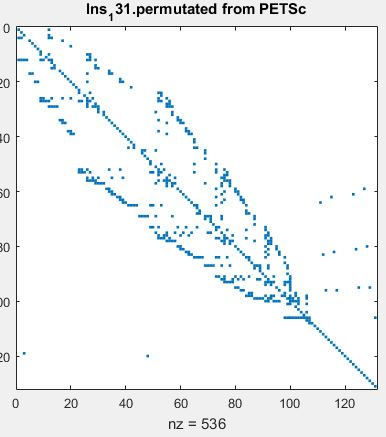
\includegraphics[width=2in]{Images/ApproxBanded_v2.jpg}
\caption{$P^TAP$ narrow band+low rank}
\label{fig:approxbanded}
\end{minipage}
\end{figure}


%\begin{figure}[ht]
%\centering
%\begin{minipage}[b]{0.45\linewidth}
%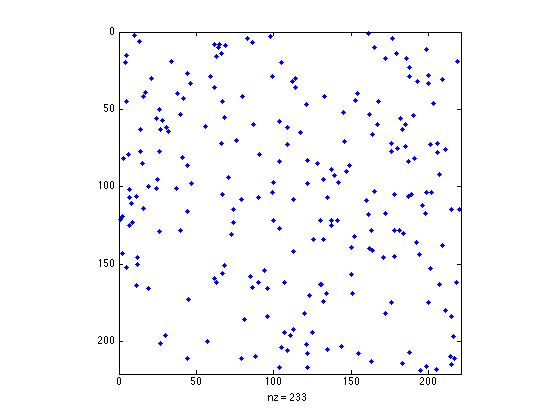
\includegraphics[width=2in]{Images/SparseA.jpg}
%\caption{$A$ is sparse and non-symmetric}
%\end{minipage}
%\quad
%\begin{minipage}[b]{0.45\linewidth}
%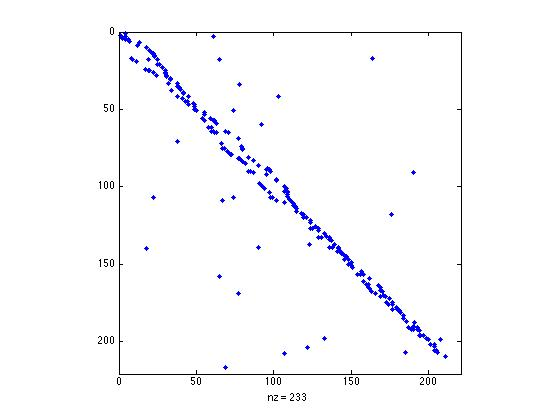
\includegraphics[width=2in]{Images/ApproxBanded.jpg}
%\caption{$P^TAP$ narrow band + low rank}
%\end{minipage}
%\label{fig:bandedplus}
%\end{figure}

\begin{figure}[htbp] %  figure placement: here, top, bottom, or page
   \centering
   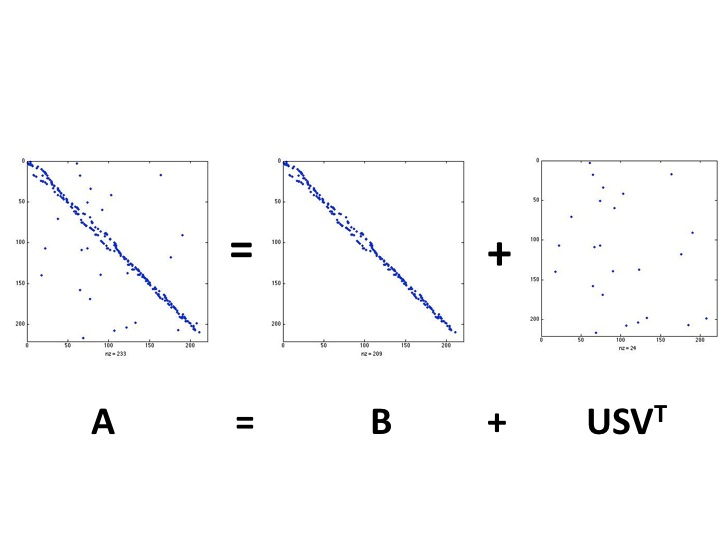
\includegraphics[trim = 5mm 30mm 0mm 40mm, clip, width=4in]{Images/Slide1.jpg}
    \caption{Breaking up $A$ into a banded matrix plus a low rank matrix}
    \label{fig:woodbury}
\end{figure}

In this case we use the Woodbury Formula to solve $Ax = b$. Recall first that $ Ax = b$  implies $x = A^{-1} b$. Then,
%\begin{block}{Woodbury Formula}
\begin{align*}
A^{-1} &= (B - USV^T)^{-1}\\
	  &= B^{-1} - B^{-1}UTV^TB^{-1}
\end{align*}
where $T = (V^TB^{-1}U - S^{-1})^{-1}$. And 
%\end{block}
\begin{align*}
x &= A^{-1}b\\
  &= {\bf B^{-1} b} - B^{-1}UTV^T {\bf B^{-1} b} \\
   &= {\bf a} - B^{-1}UT(V^T {\bf a}) \\
   &= {\bf a} - B^{-1}UT {\bf c}  \hspace{.5cm} \mbox{( solve ($V^TB^{-1}U-S^{-1}) \textbf{d} = \textbf{c}$)}\\
   &= {\bf a} - B^{-1}U\textbf{d}\\
   &= {\bf a} - B^{-1}\textbf{h}
\end{align*}

The Woodbury formula is useful because all systems involving $B$ are relatively easy to solve. We did not implement the Woodbury formula in our experiments, due to time contraints. This means that we transformed $A$ to a completely banded matrix, no matter how large the band size. We expect there would be improvements in our final results if the Woodbury formula was implemented.

In table \ref{tab:Bandsize}, the band size after permutation is shown. Matlab performed the best across the board, but all three permutations did well for our largest test case. You can see also that for the bayer01 matrix, our band size is very large, and so we did not get reasonable results in our parallel Kaczmarz implementation.

\begin{table}
\begin{center}
\begin{tabular}{| l | l | c  c  c |}
\hline

    matrix           & size         &    Matlab & PETSc     &  rcm.cpp        \\
 \hline
 lns                   & 131             &     32        &       \color{red} $\times$ 111         & \color{red} $\times$ 113  \\
 Jac2-db            & 21,982     &         545       &     \color{red} $\times$            &  \color{red} $\times$  \\
 bayer01           & 57,735      &     \color{red} $\times$ 18,322        &     \color{red} $\times$     &  \color{red} $\times$   \\
 venkat25         & 62,424      &     1,515        &    1,515    & 1,495                   \\
 stomach          & 213,360    &      1,133      & 2,216 & 2,239                    \\
 atmosmodd     & 1,270,432 &    7,772       & 7,772&  7,772                   \\
 \hline

\end{tabular}
\caption{Bandsize after RCM using various codes}
\label{tab:Bandsize}
\end{center}

\end{table}


%------------------------------------------------
%------------------------------------------------
%KACZMARZ
% NEEDS SOME RE-WRITING
%------------------------------------------------
%------------------------------------------------
% 
\subsection{The Kaczmarz method}

Once we have a banded matrix, $A$, we move on to the Kaczmarz algorithm, which was introduced earlier. Suppose we partition $A$ into two pieces $$A = \begin{pmatrix} A_1^T \\ A_2^T \end{pmatrix}  $$ and we also partition the right hand size vector $f^T = (f_1^T, f_2^T)$.


In the classical Kaczmarz method at each iteration we compute:
$$x_k=x_k+\overrightarrow{n_k}=x_k+\frac{r_k^i}{||A_i||^2}A_i^T$$
where  $\overrightarrow{n_k}=\bigtriangleup{x_k}cos\theta=\frac{\langle\,A_i{,}\,\bigtriangleup{x_k}\rangle}{||A_i||^2}A_i^T=\frac{b_i-\langle\,A_i{,}\,x_k\rangle}{||A_i||^2}A_i^T=\frac{r_k^i}{||A_i||^2}A_i^T$.
$$
\left\{
\begin{array}{ll}
                  AA^Ty = f\\
                  x = A^Ty\\
 \end{array}
 \right.
 \implies AA^T = \begin{pmatrix} A_1^T \\ A_2^T \end{pmatrix} \begin{pmatrix} A_1, A_2 \end{pmatrix}
  $$
  
  From Gauss-Seidel, use $x^{k+1} = \begin{pmatrix} A_1, A_2 \end{pmatrix} \begin{pmatrix} y_1^{k+1} \\ y_2^{k+1} \end{pmatrix} $.
  
  $$ \begin{pmatrix} A_1^TA_1 & 0 \\ A_2^T A_1 & A_2^T A_2 \end{pmatrix} \begin{pmatrix} y_1^{k+1} \\ y_2^{k+1} \end{pmatrix} =  \begin{pmatrix} 0 & -A_1A_2 \\ 0 & 0\end{pmatrix} + \begin{pmatrix} y_1^{k+1} \\ y_2^{k+1} \end{pmatrix}\begin{pmatrix} f_1 \\ f_2 \end{pmatrix}$$
  
  Replacing some parameters with projection operator $P_i$, we can get:
  $$x^{k+1} = A_1y_1^{k+1} + A_2y_2^{k+1} = Qx_k +b$$ where $Q = (I-P_2)(I-P_2)$. Similarly, for an m-partition, $$x^{k+1} = Q_u x^k + f_u = (I-P_m)(I-P_{m-1}) \ldots (I-P_1)x^k + f_u$$.
  
  However, the spectral radius of $Q_u$ may interfere with the convergence speed, and the distribution of eigenvalues could also influence the performance. To handle this, we can symmetric $Q_u$ to get an accelerated iteration: 
  $$ x^{k+1} = Q(\omega)x^k + Tf$$ where $Q(\omega) = (I-\omega P_1)(I-\omega P_2) \ldots (I-\omega P_m) \ldots (I-\omega P_2) (I-\omega P_1)$. Since $I-Q(\omega)$ is symmetric positive definite. The conjugate gradient method is suitable to accelerate the basic scheme. 
  
 Once we have a banded matrix, we considered using various partitions of the rows. A very simple example is shown in figure \ref{fig:permutation}. A permutation like this gives several benefits. The first is that we can have an outer level of parallelism for each projection. Also, when we split the matrix this way we create several small independent least squares problems, which reduces the time. 
 
 \begin{figure}[htbp]
\begin{minipage}[b]{1\linewidth}
\centering
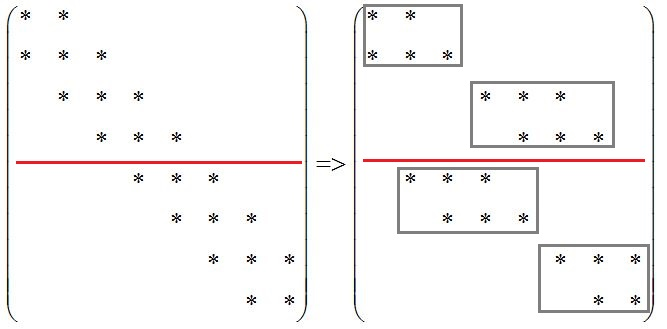
\includegraphics[width=4in]{Images/permutation}
\end{minipage}
\caption{Re-ordering the banded matrix}
\label{fig:permutation}
\end{figure}
 
 In figure \ref{fig:quality} we consider different types of partitions, both in the inner and outer levels. We found that have more independent blocks resulted in faster implementation of Kaczmarz. We also found that more partitions, i.e. taking 4 partitions: $$A = \begin{pmatrix} A_1^T  \\A_2 ^T \\ A_3^T \\ A_4^T \end{pmatrix} $$ instead of 2 partitions is slower. 
  To further illustrate this, it proved that the optimal value of $\omega$ is 1.0 if we use two partitions, and $Q(1)$ has the minimal spectral radius. For these reasons we decided to use 2 outer partitions for our implementation. In this case the problem can be simplified as follows: $$(I-Q(1))x = Tf$$


\begin{figure}[ht]
\begin{centering}
%\begin{minipage}[b]{1\linewidth}
\includegraphics[width=7in]{Images/quality.jpg}
%\end{minipage}
\end{centering}
\label{fig:quality}
\end{figure}


%\begin{figure}[ht]
%\centering
%\begin{minipage}[b]{1.0\linewidth}
%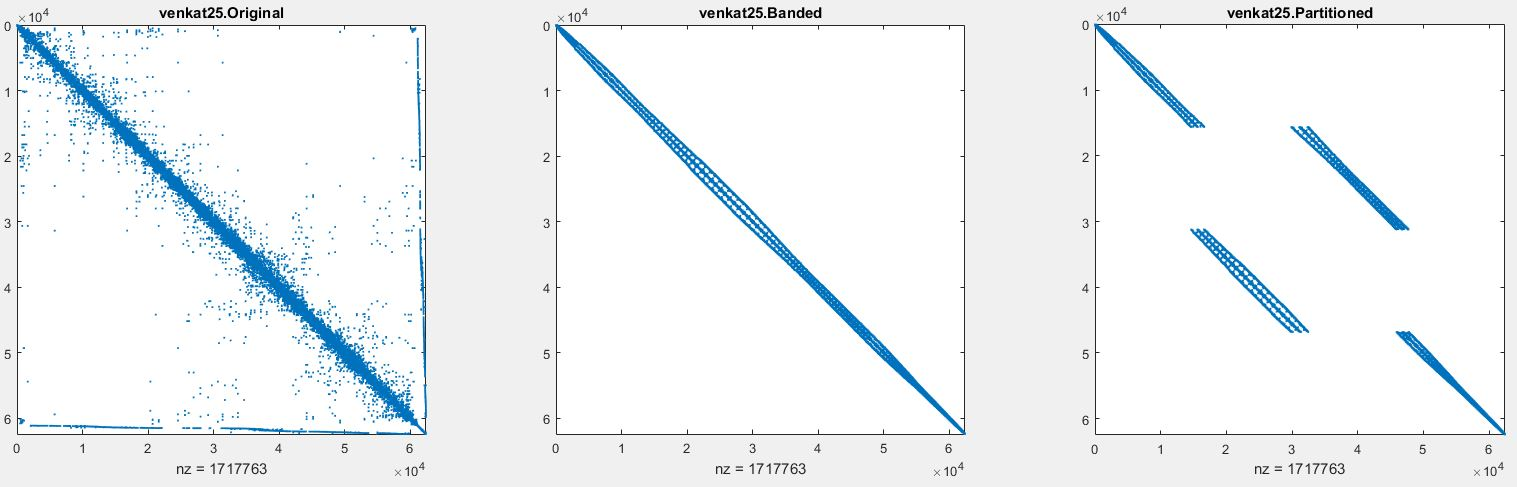
\includegraphics[width=4.8in]{Images/permute.jpg}
%\caption{$A$ is partitioned into 2 parts with several independent submatrices}
%\end{minipage}
%\end{figure}


%------------------------------------------------
%------------------------------------------------
% SYMMETRIZE KACZMARZ
% NEEDS SOME HELP
%------------------------------------------------
%------------------------------------------------
\subsection{Symmetrized Kaczmarz}
Unfortunately, the spectral radius of $Q$ may interfere with the convergence speed and the distribution of eigenvalues could also influence the performance. To handle this, we can symmetrize $Q$ to get an accelerated iteration. In our symmeterized version, we wish to solve $(I-Q)x = c$, where $c = Tf$, and $$Q=(I-P_{1})(I-P_{2})\cdot\cdot\cdot(I-P_{m})^{2}\cdot\cdot\cdot(I-P_{2})(I-P_{1})$$
 with $P_{i}=A_{i}(A_{i}^{T}A_{i})^{-1}A_{i}^{T}$, and  $T=A^{T}(D+L)^{-T}D(D+L)^{-1}$.

The algorithm to solve this system follows:

  \begin{itemize}
      \item Step1: chose $x_{0}$; set $k=0$.
      \item Step2: Compute $x_{k}=Qx_{k}$.
            \begin{equation*}
                \begin{split}
                    x_{k}=(I-P_{i})x_{k}, \quad i=1,2,...,m-1,m,m-1,...,2,1
                \end{split}
            \end{equation*}
      \item Step3: $x_{k}=x_{k}+c;$
      \item Step4: If a convergence criterion is satisfied, terminate the iterations; else set k=k+1 and go to Step2.
  \end{itemize}

It is not stable to form $P_{i}$ directly since it will square the condition number of $A_{i}$, and at the same time will cost time on solving $(A^{T}_{i}A_{i})^{-1}$. Instead, given a vector $u$ obtain $v=(I-P_{j})u \Leftrightarrow \min\limits_{v}||u-A_{j}w||_{2}$. Then solve $\min\limits_{v}||u-A_{j}w||_{2}$ directly. 
% Normal equation is unstable, QR decomposition and SVD decomposition are too slow.

In Petsc, we use CG method on normal equation: $A_{j}^{T}A_{j}w=A_{j}^{T}u$. The parallel step is:
        \begin{equation*}
            \begin{split}
                v&=\min\limits_{v}||u-A_{j}w||_{2}\Leftrightarrow \min\limits_{v_{i}}||u_{i}-A_{j,i}w_{i}||_{2},\\
                v&^{T}=[v_{1}^{T},v_{2}^{T},...,v_{k}^{T}],\\
                w&^{T}=[w_{1}^{T},w_{2}^{T},...,w_{k}^{T}].
            \end{split}
        \end{equation*}

 
 %------------------------------------------------
%------------------------------------------------
% ACCELERATION VIA CG
%MAYBE NEEDS SOME HELP
%------------------------------------------------
%------------------------------------------------

 \subsection{Acceleration via the CG Method}
As stated previously, since $(I-Q)$ is symmetric positive definite, we accelerate solving: $$(I-Q)x = Tf$$  using the conjugate gradient method. This is the framework of our entire algorithm. The outline follows:

\vspace{.2in}
 \noindent \textbf{Step 1} : $x_0 = c$ \\
\hspace{.5in} Compute $r_0 = Tf - \boxed{(I-Q)c} = Qc$\\
\hspace{.5in} Set $p_0 = r_0, i = 0$ \\
\textbf{Step 2}:  Compute: \\
\hspace{.5in} $\alpha_i = (r_i, r_i)/(p_i,\boxed{(I-Q)p_i})$ \\
\hspace{.5in} $ x_{i+1} = x_i + \alpha_i p_i $ \\
\hspace{.5in} $\beta_i = (r_{i+1}, r_{i+1})/(r_i, r_i) $ \\
\hspace{.5in} $p_{i+1} = r_{i+1} + \beta_i p _i $ \\
\textbf{Step 3}: If convergence criterion is satisfied, terminate the iterations; else set $i = i+1$ and return to Step 2.

 We can take a convergence criterion as : $$ \frac{ ||r_i||}{||r_0||} \leq \epsilon$$


The boxed out portions in our framework are very important. Remember that whenever we see: $$(I - Q) u$$ for any vector $u$, we really mean to solve multiple least squares problems:
$$(I-Q) u = (I-P_1)(I-P_2)(I-P_1) u $$
$$(I-P_i) u \Rightarrow \text{min}_{v} ||u-A_i w|| $$

 %------------------------------------------------
%------------------------------------------------
% LSQR
%------------------------------------------------
%------------------------------------------------
\subsection{LSQR}
In the end, in order to solve the least squares problem, we implemented LSQR. LSQR is an iterative method for solving $Ax = b$ where $A$ is large, sparse, and overdetermined. It is equivalent at each iteration to CG. 


\begin{algorithm}
\caption{LSQR}
\begin{algorithmic}[1]
%\Require{$P_1$ an initiator matrix; $n$, where we want to use $P_n$}
\State{$\beta_{1}u_{1}=b, \alpha_{1}v_{1}=A^{T}u_{1}, w_{1}=v_{1}, x_{0}=0, \bar{\phi_{1}}=\beta_{1},\bar{\rho_{1}}=\alpha_{1}$}
\For{$i = 1,2,3,\cdots$}
\State{Bidiagonalization:}
\State{$\beta_{i+1}u_{i+1}=Av_{i}-\alpha_{i}u_{i}$}
\State{$\alpha_{i+1}v_{i+1}=A^{T}u_{i+1}-\beta_{i+1}v_{i}$}
\State{Orthogonal Transformation:}
\State{$\rho_{i}=\sqrt{(\bar{\rho_{i}^2}+\beta_{i+1}^2)}$}
\State{$c_{i}=\bar{\rho_{i}}/\rho_{i},$}
\State{$s_{i}=\beta_{i+1}/\rho_{i},$}
\State{$\theta_{i+1}=s_{i}\alpha_{i+1},$}
\State{ $\bar{\rho_{i+1}}=-c_{i}\alpha_{i+1},$}
\State{$\phi_{i}=c_{i}\bar{\phi_{i}},$}
\State{$\bar{\phi_{i+1}}=s_{i}\bar{\phi_{i}}.$}
\State{Update x:}
\State{$x_{i}=x_{i-1}+(\phi_{i}/\rho_{i})w_{i},$}
\State{$w_{i+1}=v_{i+1}-(\theta_{i+1}/\rho_{i})w_{i}.$}
\EndFor

\end{algorithmic}
\end{algorithm}



    \begin{figure}[htbp]
    \begin{center}
        %\begin{minipage}[b]{0.8\linewidth}
            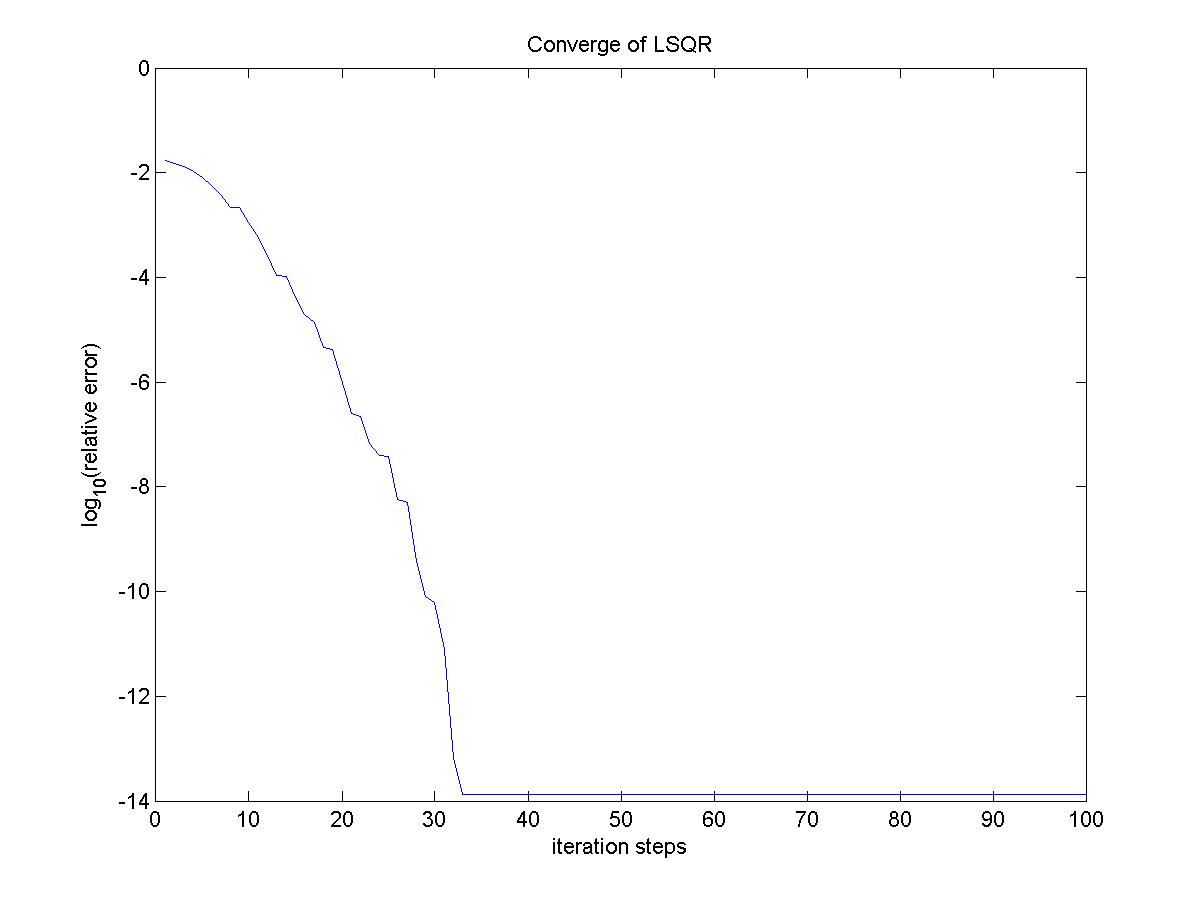
\includegraphics[width=5in]{Images/LSQR}
        %\end{minipage}
        \caption{Convergence of LSQR}
        \label{fig:LSQR}
        \end{center}
    \end{figure}





 %------------------------------------------------
%------------------------------------------------
% LAST SECTION: RESULTS
%------------------------------------------------
%------------------------------------------------

\section{Results and Conclusions}
\subsection{Results}

We will now discuss the results of our Parallel Solver. In figure \ref{fig:smallcases}, we show the run-times for 3 smaller test-cases. The x-axis shows the number of MPI-processes, while the y-axis is the run-time in seconds. We see that we do have decent scalability up to 4 nodes. At 8 nodes we do not see much improvement, or have a longer run-time. There are many reasons this could be. Our method is implemented in Petsc which is not optimized for efficiency. Also there may be too much communication in our method to fully take advantage of 8 nodes. We get similar results for our largest test-case, shown in figure \ref{fig:largestcase}.

Note: these results are the time taken to converge to with a tolerance of $10^{-8}$.


\begin{figure}[h] %  figure placement: here, top, bottom, or page
   \centering
   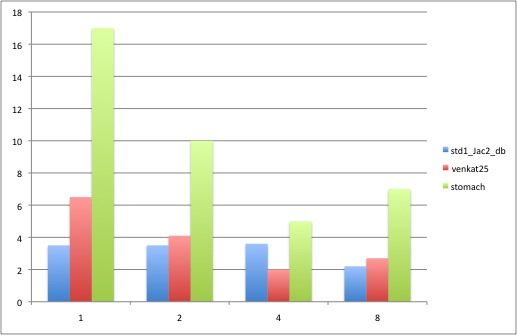
\includegraphics[width=5in]{Images/runtimes.jpg}
   \caption{std1\_Jac2bd: $n = 21982$; venkat25: $n=62424$, stomach: $n=213360$.}
   \label{fig:smallcases}
\end{figure}


\begin{figure}[h] %  figure placement: here, top, bottom, or page
   \centering
   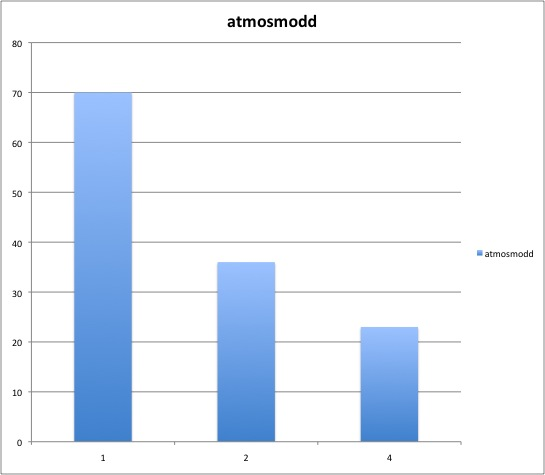
\includegraphics[width=4in]{Images/atmosmodd.jpg}
   \caption{Runtime in seconds for largest test case ($n = 1270432$).}
   \label{fig:largestcase}
\end{figure}



To find a benchmark of how well our method performed, we compared with a Krylov Subspace method. The implementation of this consisted of first using the MC64 software to re-order the matrix. This software finds a permutation which brings non-zeros to the diagonal. Once this permutation is used, then we called a Krylov Subspace method with ILU pre-conditioner in Petsc. The Krylov subspace method used is GMRES.

We quickly realized that the ILU preconditioner failed on some of our data. The reason for this could be that the eigenvalues of these matrices are distributed too much across the positive and negative spectrum. The ILU preconditioner is not well equipped to handle these so called ``highly indefinite'' matrices. Table \ref{tab:MC64} shows which of our data failed with this method.
\begin{table}
\begin{center}
\begin{tabular}{| l | l | c |}
\hline
matrix             & size        & Converged? \\
\hline
lns                  & 131         &    \color{red} $\times$  \\
std1-Jac2-db  & 21,982    & \color{red}  $\times$  \\
bayer01          & 57,735    &  \color{red} $\times$   \\
venkat25        & 62,424     & \color{green} \Checkmark   \\
stomach         & 213,360   &  \color{green}  \Checkmark  \\
atmosmodd    & 1,270,432 &  \color{green} \Checkmark  \\
\hline
\end{tabular}
\end{center}
\caption{ILU preconditioner}
\label{tab:MC64}
\end{table}


Finally, we compared the run-time of this Krylov method to our results on 4 MPI processors. We compared both the number of iterations and the time to converge to a tolerance of $10^{-8}$. The results are shown in Table \ref{tab:finalresults}. Overall our parallel solver out-performs the Krylov Subspace Method. The data set Stomach is an exception; this data set has very nice properties that allows the Krylov Method to converge very fast.
\begin{table}
\begin{center}
\begin{tabular}{| l | l | c  c | c  c |}
\hline
                         &                & Our Parallel & Solver & Krylov & ILU\\
                          \hline
    matrix           & size         &    num-its & time (s)     &  num-its & time (s)        \\
 \hline
 lns                   & 131             &     10   &         .1  & \color{red} $\times$  &  \color{red} $\times$\\
 Jac2-db            & 21,982     &    13     &     .8      &  \color{red} $\times$  & \color{red} $\times$ \\
 bayer01        & 57,735  &  \color{red} $\times$    &   \color{red} $\times$    &  \color{red} $\times$  & \color{red} $\times$ \\
 venkat25         & 62,424      & 12     &     1.5   & 374                   & 14.17 \\
 stomach          & 213,360    &   15    & 4 & 16                   & 2.21 \\
 atmosmodd     & 1,270,432 &  14    &  21 &  266                   & 130.72 \\
 \hline

\end{tabular}
\end{center}
\caption{Run times for 4 MPI Processors to converge with tol = $10^{-8}$}
\label{tab:finalresults}
\end{table}


\subsection{Conclusions}
In conclusion, it was a mistake to use Petsc. Petsc is better for high level implementation, not for optimization and efficiency. Petsc was also not well suited specifically for grabbing the exact sub-matrices that we needed in order to call the parallel Least Squares. 

In the end we were able to salvage our project by implementing LSQR, which greatly reduced our run-time and even produced some nice scalability. Even so, if we had left Petsc out of our project we believe our results would have been even better.



\end{document}


